\newpage
\section{Produktfunktionen}
Es werden die Funktionen anhand von verschieden Kriterien beschrieben. Diese können im genaueren aus der unteren Tabelle entnommen werden.
\UseCase{
	{Der Bereich, unter welchen die Funktionen fällt}
	{Der Name und die ID der Funktion}
	{Die Art, unter welche die Funktion in dessen Umsetzung fallen wird}
	{Eine kurze Beschreibung der Funktion.}
	{Der Grund für die Existenz der Funktion im Produkt.}
	{Das Ergebnis, welche die Funktion erfüllen soll.}
	{Die verschiedenen Teilnehmer, welche von dieser Funktion betroffen sind.}
	{Die ein- und ausgehenden Informationen welche in Zusammenhang mit dieser Funktion stehen.}
	{Die Bedingungen, welche von dem Eintreffen der Funktion herrschen.}
	{Die Bedingungen, welche nach dem Eintreffen der Funktion herrschen.}
	{Der Nutzen der Funktion: gering, mittel, hoch}
	{Der Aufwand der Funktion: gering, mittel, hoch}
	{Die Priorität der Funktion: Must Have, Should Have, Nice to Have}
}

\subsection{Desktop-Version}
Es werden die Funktionen beschrieben, welche die Desktop-Version des Produktes erfüllen soll. Diese werden grundsätzliche in Frontend und Backend unterteilt.
\subsubsection{Backend erstellen}
Das Backend umfasst alle Funktionen, welche vom Benutzer nicht gesehen werden können. Diese bearbeitet den Datentransfer, Datenaufbereitung und die Datensicherheit.
\paragraph{Aktivitätsdiagramm Backend}\mbox{}\\
\begin{figure}[H]
	\centering
	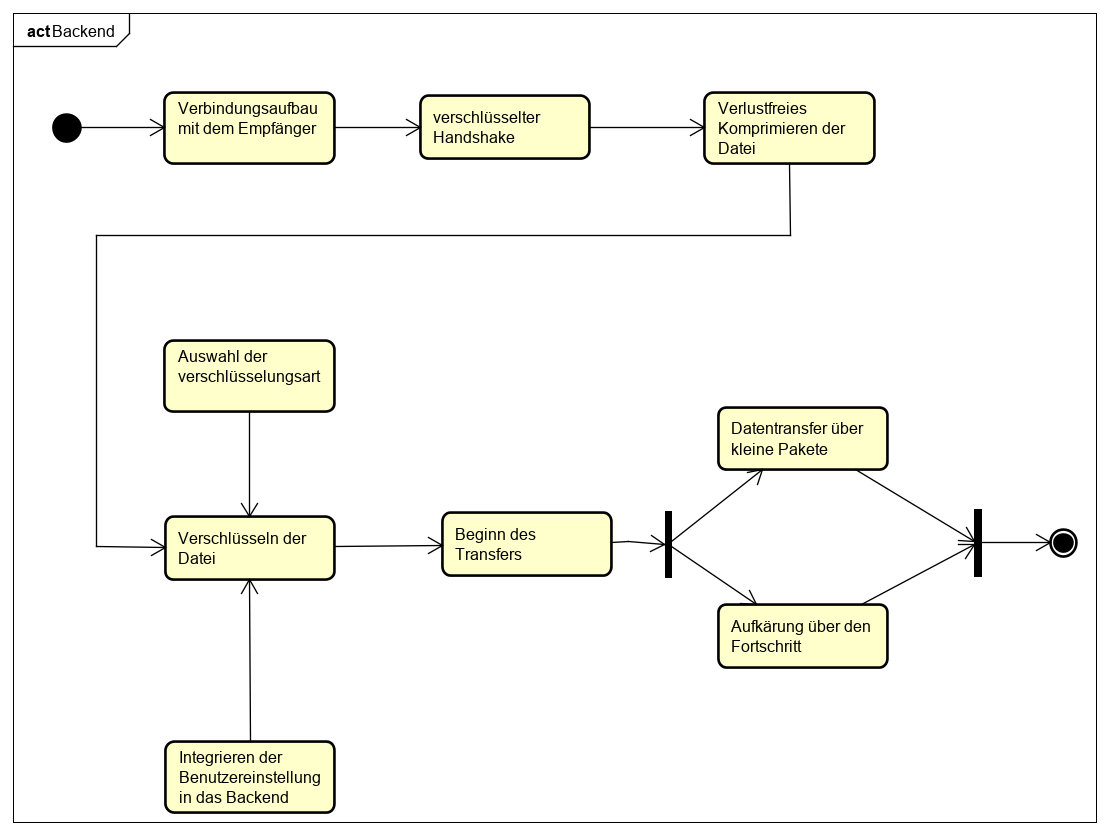
\includegraphics[width= 0.9\linewidth]{diagramms/activity/Backend.png}
	\caption{Aktivitätsdiagramm Backend}
\end{figure}
\newpage
\begin{indentE}\mbox{}
	\paragraph{/LF1110/ Verbindung aufbauen}\mbox{}\\
	Es wird die Verbindung mit dem ausgewählten Empfänger aufgebaut. Dieser Verbindungsaufbau besteht aus einem verschlüsselten Handshake, mit welchem die Systemdaten des Empfängers und Senders ausgetauscht werden. Wenn Empfänger und Sender den selben Verschlüsselungsschlüssel gewählt haben, ist der Handshake erfolgreich und der Transfer kann beginnen.
	\UseCase{
		{Desktop Backend}
		{/LF1110/ Verbindung aufbauen}
		{Backend}
		{Es wird die Verbindung mit dem Empfänger als Sender aufgebaut.}
		{Es muss eine Verbindung zwischen Empfänger und Sender für den Datentransfer herrschen}
		{Der Empfänger kann sich mit einem Empfänger der Wahl verbinden.}
		{Empfänger, Sender}
		{Sender, Namen }
		{Der Sender kann sich nicht mit dem Empfänger verbinden.}
		{Der Sender kann sich mit dem Empfänger verbinden.}
		{hoch}
		{mittel}
		{Must Have}
	}
	\paragraph{/LF1120/ Daten transferieren}\mbox{}\\
	Die Daten werden in kleinen Paketen versandt, um die Datensicherheit zu garantieren. Dabei haben diese eine einheitliche Größe und es werden unterschiedliche viele je nach Datengröße versandt. Dabei sollen der Empfänger und der Sender um den Fortschritt der Übertragung aufgeklärt werden.
	\UseCase{
		{Desktop Backend}
		{/LF1120/ Daten transferieren}
		{Backend}
		{Die Daten sollen vom Sender zum Empfänger transferiert werden. Diese soll dabei möglichst verlustlos gesendet werden.}
		{Der Daten müssen an den Empfänger gebracht werden.}
		{Die Daten des Sender kommen beim Empfänger an.}
		{Empfänger, Sender}
		{Datei(Name, Größe, Inhalt), Fortschritt(aus index und Anzahl Pakete), Sender, Empfänger}
		{Die Daten können dem Empfänger nicht vom Sender geschickt werden.}
		{Die Daten werden vom Sender zum Empfänger verlustlos gesendet.}
		{hoch}
		{gering}
		{Must Have}
	}
	\paragraph{/LF1130/ Daten komprimieren}\mbox{}\\
	Die Daten werden vor dem Versand verlustlos komprimiert, um die Datenmenge zu verkleinern. Die dabei gewählt Komprimierungsart, darf vom Auftragnehmer ausgewählt werden.
	\UseCase{
		{Desktop Backend}
		{/LF1130/ Daten komprimieren}
		{Backend}
		{Die Daten sollen vor dem Transfer verlustlos komprimiert werden, um die Übertragungsdauer zu verringern}
		{Der Datentransfer soll kürzer dauern.}
		{Der Datentransfer dauert in den meisten Fällen kürzer.}
		{Sender, Empfänger}
		{Daten}
		{Die Datenübertragung dauert länger.}
		{Die Datenübertragung dauert kürzer.}
		{mittel}
		{mittel}
		{Should Have}
	}
	\paragraph{/LF1140/ Datentransfer verschlüsseln}\mbox{}\\
	Der Datentransfer wird mit einem Verschlüsselungsschlüssel nach dem AES256 Standard verschlüsselt, um die Datensicherheit zu erhöhen. Diese wird dann vom Empfänger wieder entschlüsselt. Die dafür benutzte Verschlüsselungsart, kann vom Auftraggeber ausgewählt werden.
	\UseCase{
		{Desktop Backend}
		{/LF1140/ Datentransfer verschlüsseln}
		{Backend}
		{Der Datentransfer soll für eine höhere Sicherheit durch einen Schlüssel verschlüsselt werden.}
		{Der Datentransfer soll verschlüsselt stattfinden, damit die originalen Daten nicht von Dritten ausgelesen werden können.}
		{Der Datentransfer erfüllt den Standard AES256.}
		{Empfänger, Sender, Dritte}
		{Daten, Schlüssel}
		{Die originalen Daten können von Dritten ausgelesen werden}
		{Die originalen Daten sind während dem Transfer verschlüsselt}
		{mittel}
		{mittel}
		{Must Have}
	}
	\paragraph{/LF1150/ Benutzereinstellungen integrieren}\mbox{}\\
	Die vom Benutzer ausgewählten Benutzereinstellungen müssen in das Backend integrierte werden, um den Nutzen aus diesen Werten zu ziehen.
	\UseCase{
		{Desktop Backend}
		{/LF1150/ Benutzereinstellungen integrieren}
		{Backend}
		{Die Benutzereinstellungen sollen integriert werden.}
		{Die ausgewählten Benutzereinstellungen sollen in das Backend integriert werden.}
		{Die Einstellungen des Benutzer haben eine Auswirkung auf das Backend.}
		{Sender, Empfänger}
		{gewünschte Systemname, Verschlüsselung (Ja/Nein), Standardschlüssel, Speicherort}
		{Der Benutzer muss die meisten Daten bei jeder Übertragung neu einstellen, wodurch diese länger dauert}
		{Der Übertragung ist anpassbar, wodurch diese verschnellert werden kann. }
		{mittel}
		{gering}
		{Should Have}
	}
\end{indentE}
\subsubsection{Frontend erstellen}
Zu dem Frontend des Produktes gehören alle Elemente, auf welche der Benutzer Einsicht hat und mit denen er interagieren kann. Diese sind besonders für die Benutzbarkeit des Produkt wichtig, da diese die wichtigste Produktqualität ist.
\paragraph{Aktivitätsdiagramm Frontend}\mbox{}\\
\begin{figure}[H]
	\centering
	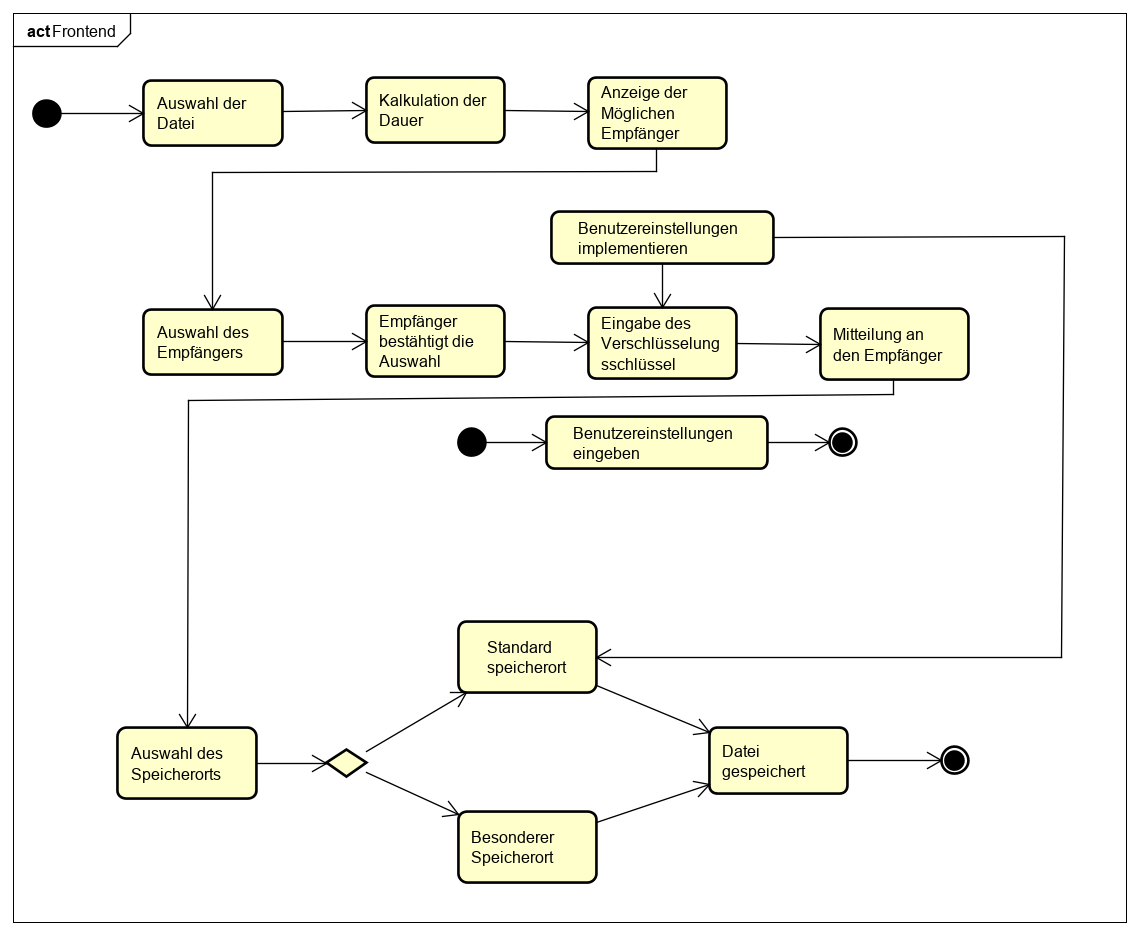
\includegraphics[width= 0.9\linewidth]{diagramms/activity/Frontend.png}
	\caption{Aktivitätsdiagramm Frontend}
\end{figure}
\newpage
\begin{indentE}\mbox{}
	\paragraph{/LF1210/ Datei auswählen}\mbox{}\\
	Der Benutzer wählt eine Datei aus, welche er verschicken möchte. Hierbei soll eine voreilige Kalkulation durchgeführt werden, welche die Dauer der Übertragung schätzt.
	\UseCase{
		{Desktop Frontend}
		{/LF1210/ Datei auswählen}
		{Frontend}
		{Ein wird die zu versendende Datei ausgewählt.}
		{Es muss die Datei, welche versendet werden soll, ausgewählt werden}
		{Es kann die Datei gesendet werden}
		{Sender}
		{Datei(Name, Größe, Inhalt)}
		{Es kann keine Datei ausgewählt werden}
		{Es kann eine zu versendende Datei ausgewählt werden}
		{hoch}
		{mittel}
		{Must Have}
	}
	\paragraph{/LF1220/ Empfänger auswählen}\mbox{}\\
	Es werden dem Benutzer die möglichen Empfänger angezeigt und ausgwählt oder er kann den Namen des Empfängers eingeben, um den Empfänger zu bestimmen. Dieser muss die Verbindung bestätigen.
	\UseCase{
		{Desktop Frontend}
		{/LF1220/ Empfänger auswählen}
		{Frontend}
		{Der Sender wählt anhand des Namens den Empfänger aus, mit dem der Datentransfer stattfinden soll.}
		{Es muss der Empfänger ausgewählt werden.}
		{Die Verbindung kann aufgebaut werden}
		{Sender, Empfänger}
		{Sendername, Empfängername}
		{Es kann kein Empfänger ausgewählt werden.}
		{Es kann anhand des Namens der Empfänger der Datei ausgewählt werden.}
		{hoch}
		{mittel}
		{Must Have}
	}
	\paragraph{/LF1230/ Verschlüsselungsschlüssel eingeben}\mbox{}\\
	Wenn kein Standard-Schlüssel ausgewählt ist, muss der Sender diesen bevor dem Verbindungsaufbau eingeben. Dieser muss dann dem Empfänger mitgeteilt werden und dieser muss den selben auch eingeben, um den Datentransfer zu ermöglichen.
	\UseCase{
		{Desktop Frontend}
		{/LF1230/ Verschlüsselungsschlüssel eingeben}
		{Frontend}
		{Es müssen Empfänger und Sender einen Schlüssel eingeben, die übereinstimmen, um den Datentransfer zu beginnen.}
		{Der Datentransfer muss mit einem Schlüssel verschlüsselt werden.}
		{Der Datentransfer kann verschlüsselt werden}
		{Sender, Empfänger}
		{Schlüssel}
		{Die Daten können nicht mit einem Schlüssel verschlüsselt werden}
		{Die Daten können mit einem frei wählbaren Schlüssel verschlüsselt werden}
		{hoch}
		{mittel}
		{Must Have}
	}
	\paragraph{/LF1240/ Datei speichern}\mbox{}\\
	Der Empfänger soll nach dem empfangen der Datei auswählen können, ob diese im Standard-Speicherort gespeichert wird, oder in einem besonderen. Wenn der Besondere ausgewählt worden ist, soll ihm ein Benutzerinterface gezeigt werden, indem er den Speicherort auswählen.
	\UseCase{
		{Desktop Frontend}
		{/LF1240/ Datei speichern}
		{Frontend}
		{Der Empfänger soll den Speicherort des bekommenen Datei auswählen können.}
		{Die Datei muss irgendwo gespeichert werden}
		{Der Speicherort der Datei kann ausgewählt werden}
		{Empfänger}
		{Datei(Name, Größe, Inhalt), Speicherort}
		{Die Datei wird entweder immer am selben Ort, oder nicht gespeichert}
		{Der Speicherort kann frei gewählt werden}
		{mittel}
		{gering}
		{Must Have}
	}
	\paragraph{/LF1250/ Benutzereinstellungen hinzufügen}\mbox{}\\
	Der Benutzer kann einige Fix-Einstellungen auf seinem Produkt tätigen. Darunter zählt die Möglichkeit, den Namen zu ändern, welcher den restlichen Nutzern angezeigt wird, die Verschlüsselung zu aktivieren oder deaktivieren, einen Standardschlüssel auszuwählen und einen Standard-Speicherort auszuwählen. Dabei sollen die eingegebenen Daten auf ihre Korrektheit überprüft werden.
	\UseCase{
		{Desktop Frontend}
		{/LF1250/ Benutzereinstellungen hinzufügen}
		{Frontend}
		{Der Benutzer kann verschiedenen Einstellungen tätigen, mit welche er die Datenübertragung beeinflussen kann.}
		{Die Einstellungen müssen auf einem Interface getätigt werden}
		{Die Einstellungen können getätigt werden}
		{Empfänger, Sender}
		{gewünschter Systemname, Verschlüsselung(Ja/Nein), Standardschlüssel, Standard-Speicherort}
		{Das Produkt kann nicht angepasst werden.}
		{Es können Einstellungen getroffen werden, welche das Produkt beeinflussen.}
		{mittel}
		{mittel}
		{Should Have}
	}
	\paragraph{/LF1260/ Desktopinterface designen}\mbox{}\\
	Es muss ein Interface für den Desktop entworfen werden. Dazu gehören Mockups und Prototypen. Diese müssen vor deren Implementierung vom Auftraggeber bestätigt werden.
	\UseCase{
		{Desktop Frontend}
		{/LF1260/ Desktopinterface designen}
		{Frontend}
		{Es müssen Mockups für die Desktopinterfaces erstellt werden. Diese diene als Vorlage für die Interfaces.}
		{Für einen schnellere und besser Implementierung sollen Mockups als Vorlage dienen.}
		{Die Implementierung ist einfacher, schneller und besser.}
		{Auftraggeber, Auftragnehmer}
		{}
		{Das Interface wird ohne Vorlage erstellt.}
		{Das Interface kann nach einer vom Auftraggeber bestätigten Vorlage erstellt werden.}
		{mittel}
		{gering}
		{Should Have}
	}
	\paragraph{/LF1270/ Desktopinterace implementieren}\mbox{}\\
	Das Desktopinterface muss nach der Bestätigung des Auftraggeber implementiert werden. 
	\UseCase{
		{Desktop Frontend}
		{/LF1270/}
		{Frontend}
		{Das Desktopinterface muss durch die Mockups realisiert werden.}
		{Der Benutzer hat keine Möglichkeit mit dem System zu integrieren}
		{Der Benutzer kann mit dem System interagieren und dadurch dessen Funktionen benutzen.}
		{Benutzer}
		{sämtliche Nutzereingaben}
		{Der Benutzer kann mit dem System nicht interagieren}
		{Der Benutzer ist in der Lage mit dem System zu interagieren}
		{hoch}
		{hoch}
		{Must-Have}
	}
	\paragraph{/LF1280/ Frontend und Backend verbinden}\mbox{}\\
	Es muss eine Verbindung zwischen dem Frontend und Backend erstellt werden, welche die Aufforderungen verarbeitet und zum Backend weiterleitet. Diese Verbindung, soll dem Benutzer entweder mitteilen, wie lange die Verarbeitung noch dauert oder bei kürzeren das wiederholte Aufrufen von Aufforderungen verhindern.
	\UseCase{
		{Desktop Frontend}
		{/LF1280/ Frontend und Backend verbinden}
		{Frontend}
		{Das Frontend muss mit dem Backend verbunden werden, um die Nutzereingaben an das Backend weiterzuleiten. Außerdem soll es Daten ans Frontend schicken, welche über momentane Prozess aufklärt.}
		{Die Daten müssen vom Frontend ans Backend und umgekehrt geschickt werden}
		{Das Frontend kann mit dem Backend und umgekehrt kommunizieren.}
		{Benutzer}
		{sämtliche Nutzereingaben und verwertete Daten}
		{Die Nutzerdaten können nicht an das Backend und die verwerteten Daten nicht ans Frontend geschickt werden.}
		{Daten können zwischen Frontend und Backend ausgetauscht werden.}
		{hoch}
		{mittel}
		{Must-Have}
	}
\end{indentE}
\subsection{App-Version}
Es werden die Funktionen beschrieben, welche die App-Version des Produktes erfüllen soll. Diese werden grundsätzliche in Frontend und Backend unterteilt.
\subsubsection{Backend erstellen}
Das Backend umfasst alle Funktionen, welche vom Benutzer nicht gesehen werden können. Diese bearbeitet den Datentransfer, Datenaufbereitung und die Datensicherheit.
\paragraph{Aktivitätsdiagramm Backend}\mbox{}\\
\begin{figure}[H]
	\centering
	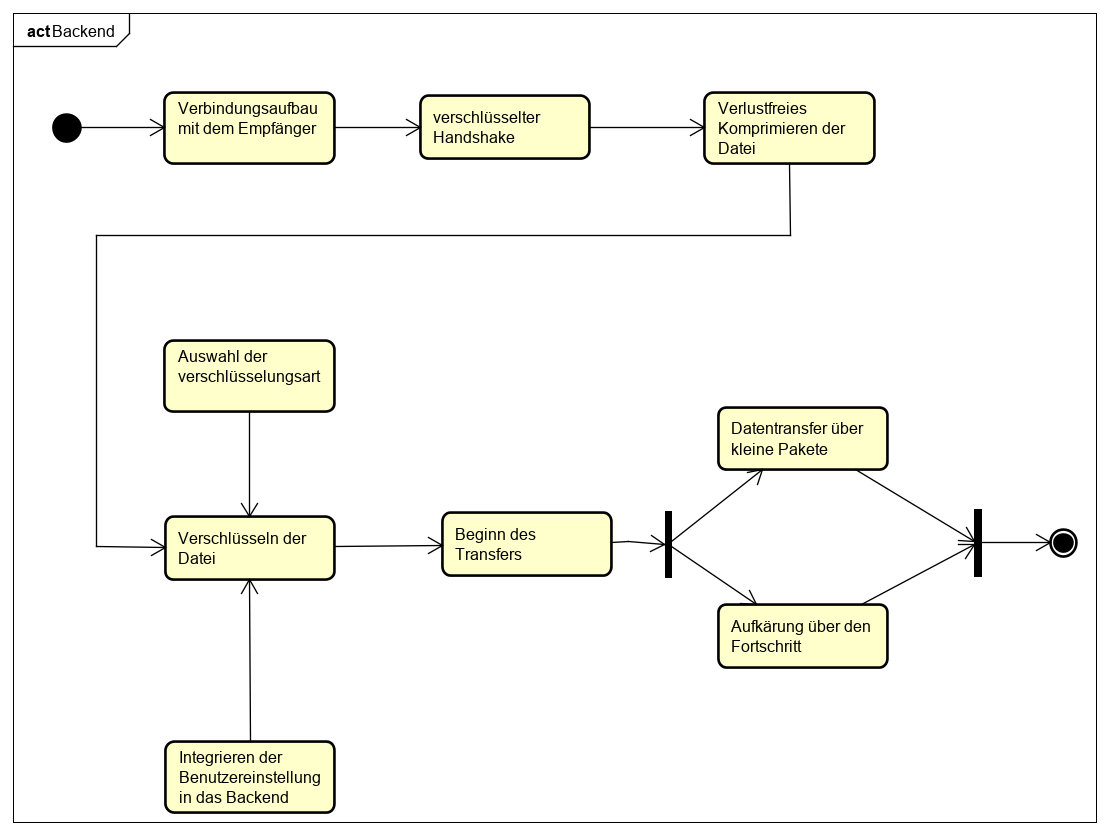
\includegraphics[width= 0.9\linewidth]{diagramms/activity/Backend.png}
	\caption{Aktivitätsdiagramm Backend}
\end{figure}
\newpage
\begin{indentE}\mbox{}
	\paragraph{/LF2110/ Verbindung aufbauen}\mbox{}\\
	Es wird die Verbindung mit dem ausgewählten Empfänger aufgebaut. Dieser Verbindungsaufbau besteht aus einem verschlüsselten Handshake, mit welchem die Systemdaten des Empfängers und Senders ausgetauscht werden. Wenn Empfänger und Sender den selben Verschlüsselungsschlüssel gewählt haben, ist der Handshake erfolgreich und der Transfer kann beginnen.
	\UseCase{
		{App Backend}
		{/LF2110/ Verbindung aufbauen}
		{Backend}
		{Es wird die Verbindung mit dem Empfänger als Sender aufgebaut.}
		{Es muss eine Verbindung zwischen Empfänger und Sender für den Datentransfer herrschen}
		{Der Empfänger kann sich mit einem Empfänger der Wahl verbinden.}
		{Empfänger, Sender}
		{Sender, Namen }
		{Der Sender kann sich nicht mit dem Empfänger verbinden.}
		{Der Sender kann sich mit dem Empfänger verbinden.}
		{hoch}
		{mittel}
		{Should Have}
	}
	\paragraph{/LF2120/ Daten transferieren}\mbox{}\\
	Die Daten werden in kleinen Paketen versandt, um die Datensicherheit zu garantieren. Dabei haben diese eine einheitliche Größe und es werden unterschiedliche viele je nach Datengröße versandt. Dabei sollen der Empfänger und der Sender um den Fortschritt der Übertragung aufgeklärt werden.
	\UseCase{
		{App Backend}
		{/LF2120/ Daten transferieren}
		{Backend}
		{Die Daten sollen vom Sender zum Empfänger transferiert werden. Diese soll dabei möglichst verlustlos gesendet werden.}
		{Der Daten müssen an den Empfänger gebracht werden.}
		{Die Daten des Sender kommen beim Empfänger an.}
		{Empfänger, Sender}
		{Datei(Name, Größe, Inhalt), Fortschritt(aus index und Anzahl Pakete), Sender, Empfänger}
		{Die Daten können dem Empfänger nicht vom Sender geschickt werden.}
		{Die Daten werden vom Sender zum Empfänger verlustlos gesendet.}
		{hoch}
		{gering}
		{Should Have}
	}
	\paragraph{/LF2130/ Daten komprimieren}\mbox{}\\
	Die Daten werden vor dem Versand verlustlos komprimiert, um die Datenmenge zu verkleinern. Die dabei gewählt Komprimierungsart, darf vom Auftragnehmer ausgewählt werden.
	\UseCase{
		{App Backend}
		{/LF2130/ Daten komprimieren}
		{Backend}
		{Die Daten sollen vor dem Transfer verlustlos komprimiert werden, um die Übertragungsdauer zu verringern}
		{Der Datentransfer soll kürzer dauern.}
		{Der Datentransfer dauert in den meisten Fällen kürzer.}
		{Sender, Empfänger}
		{Daten}
		{Die Datenübertragung dauert länger.}
		{Die Datenübertragung dauert kürzer.}
		{mittel}
		{mittel}
		{Nice to Have}
	}
	\paragraph{/LF2140/ Datentransfer verschlüsseln}\mbox{}\\
	Der Datentransfer wird mit einem Verschlüsselungsschlüssel nach dem AES256 Standard verschlüsselt, um die Datensicherheit zu erhöhen. Diese wird dann vom Empfänger wieder entschlüsselt. Die dafür benutzte Verschlüsselungsart, kann vom Auftraggeber ausgewählt werden.
	\UseCase{
		{App Backend}
		{/LF2140/ Datentransfer verschlüsseln}
		{Backend}
		{Der Datentransfer soll für eine höhere Sicherheit durch einen Schlüssel verschlüsselt werden.}
		{Der Datentransfer soll verschlüsselt stattfinden, damit die originalen Daten nicht von Dritten ausgelesen werden können.}
		{Der Datentransfer erfüllt den Standard AES256.}
		{Empfänger, Sender, Dritte}
		{Daten, Schlüssel}
		{Die originalen Daten können von Dritten ausgelesen werden}
		{Die originalen Daten sind während dem Transfer verschlüsselt}
		{mittel}
		{mittel}
		{Should Have}
	}
	\paragraph{/LF2150/ Benutzereinstellungen integrieren}\mbox{}\\
	Die vom Benutzer ausgewählten Benutzereinstellungen müssen in das Backend integrierte werden, um den Nutzen aus diesen Werten zu ziehen.
	\UseCase{
		{App Backend}
		{/LF2150/ Benutzereinstellungen integrieren}
		{Backend}
		{Die Benutzereinstellungen sollen integriert werden.}
		{Die ausgewählten Benutzereinstellungen sollen in das Backend integriert werden.}
		{Die Einstellungen des Benutzer haben eine Auswirkung auf das Backend.}
		{Sender, Empfänger}
		{gewünschte Systemname, Verschlüsselung (Ja/Nein), Standardschlüssel, Speicherort}
		{Der Benutzer muss die meisten Daten bei jeder Übertragung neu einstellen, wodurch diese länger dauert}
		{Der Übertragung ist anpassbar, wodurch diese verschnellert werden kann. }
		{mittel}
		{gering}
		{Nice to Have}
	}
\end{indentE}
\subsubsection{Frontend erstellen}
Zu dem Frontend des Produktes gehören alle Elemente, auf welche der Benutzer Einsicht hat und mit denen er interagieren kann. Diese sind besonders für die Benutzbarkeit des Produkt wichtig, da diese die wichtigste Produktqualität ist.
\paragraph{Aktivitätsdiagramm Frontend}\mbox{}\\
\begin{figure}[H]
	\centering
	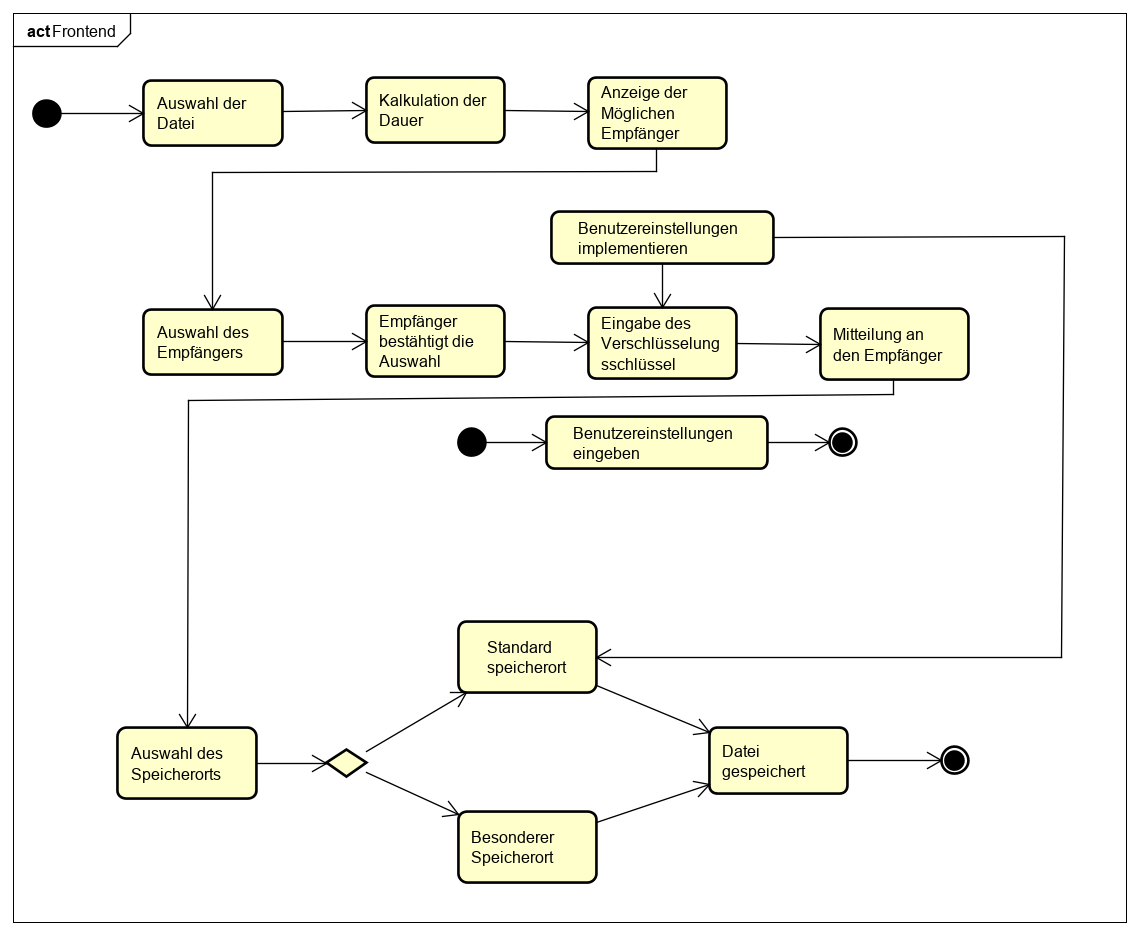
\includegraphics[width= 0.9\linewidth]{diagramms/activity/Frontend.png}
	\caption{Aktivitätsdiagramm Frontend}
\end{figure}
\newpage
\begin{indentE}\mbox{}
	\paragraph{/LF2210/ Datei auswählen}\mbox{}\\
	Der Benutzer wählt eine Datei aus, welche er verschicken möchte. Hierbei soll eine voreilige Kalkulation durchgeführt werden, welche die Dauer der Übertragung schätzt.
	\UseCase{
		{App Frontend}
		{/LF2210/ Datei auswählen}
		{Frontend}
		{Ein wird die zu versendende Datei ausgewählt.}
		{Es muss die Datei, welche versendet werden soll, ausgewählt werden}
		{Es kann die Datei gesendet werden}
		{Sender}
		{Datei(Name, Größe, Inhalt)}
		{Es kann keine Datei ausgewählt werden}
		{Es kann eine zu versendende Datei ausgewählt werden}
		{hoch}
		{mittel}
		{Should Have}
	}
	\paragraph{/LF2220/ Empfänger auswählen}\mbox{}\\
	Es werden dem Benutzer die möglichen Empfänger angezeigt und ausgwählt oder er kann den Namen des Empfängers eingeben, um den Empfänger zu bestimmen. Dieser muss die Verbindung bestätigen.
	\UseCase{
		{App Frontend}
		{/LF2220/ Empfänger auswählen}
		{Frontend}
		{Der Sender wählt anhand des Namens den Empfänger aus, mit dem der Datentransfer stattfinden soll.}
		{Es muss der Empfänger ausgewählt werden.}
		{Die Verbindung kann aufgebaut werden}
		{Sender, Empfänger}
		{Sendername, Empfängername}
		{Es kann kein Empfänger ausgewählt werden.}
		{Es kann anhand des Namens der Empfänger der Datei ausgewählt werden.}
		{hoch}
		{mittel}
		{Should Have}
	}
	\paragraph{/LF2230/ Verschlüsselungsschlüssel eingeben}\mbox{}\\
	Wenn kein Standard-Schlüssel ausgewählt ist, muss der Sender diesen bevor dem Verbindungsaufbau eingeben. Dieser muss dann dem Empfänger mitgeteilt werden und dieser muss den selben auch eingeben, um den Datentransfer zu ermöglichen.
	\UseCase{
		{App Frontend}
		{/LF2230/ Verschlüsselungsschlüssel eingeben}
		{Frontend}
		{Es müssen Empfänger und Sender einen Schlüssel eingeben, die übereinstimmen, um den Datentransfer zu beginnen.}
		{Der Datentransfer muss mit einem Schlüssel verschlüsselt werden.}
		{Der Datentransfer kann verschlüsselt werden}
		{Sender, Empfänger}
		{Schlüssel}
		{Die Daten können nicht mit einem Schlüssel verschlüsselt werden}
		{Die Daten können mit einem frei wählbaren Schlüssel verschlüsselt werden}
		{hoch}
		{mittel}
		{Should Have}
	}
	\paragraph{/LF2240/ Datei speichern}\mbox{}\\
	Der Empfänger soll nach dem empfangen der Datei auswählen können, ob diese im Standard-Speicherort gespeichert wird, oder in einem besonderen. Wenn der Besondere ausgewählt worden ist, soll ihm ein Benutzerinterface gezeigt werden, indem er den Speicherort auswählen.
	\UseCase{
		{App Frontend}
		{/LF2240/ Datei speichern}
		{Frontend}
		{Der Empfänger soll den Speicherort des bekommenen Datei auswählen können.}
		{Die Datei muss irgendwo gespeichert werden}
		{Der Speicherort der Datei kann ausgewählt werden}
		{Empfänger}
		{Datei(Name, Größe, Inhalt), Speicherort}
		{Die Datei wird entweder immer am selben Ort, oder nicht gespeichert}
		{Der Speicherort kann frei gewählt werden}
		{mittel}
		{gering}
		{Should Have}
	}
	\paragraph{/LF2250/ Benutzereinstellungen hinzufügen}\mbox{}\\
	Der Benutzer kann einige Fix-Einstellungen auf seinem Produkt tätigen. Darunter zählt die Möglichkeit, den Namen zu ändern, welcher den restlichen Nutzern angezeigt wird, die Verschlüsselung zu aktivieren oder deaktivieren, einen Standardschlüssel auszuwählen und einen Standard-Speicherort auszuwählen. Dabei sollen die eingegebenen Daten auf ihre Korrektheit überprüft werden.
	\UseCase{
		{App Frontend}
		{/LF2250/ Benutzereinstellungen hinzufügen}
		{Frontend}
		{Der Benutzer kann verschiedenen Einstellungen tätigen, mit welche er die Datenübertragung beeinflussen kann.}
		{Die Einstellungen müssen auf einem Interface getätigt werden}
		{Die Einstellungen können getätigt werden}
		{Empfänger, Sender}
		{gewünschter Systemname, Verschlüsselung(Ja/Nein), Standardschlüssel, Standard-Speicherort}
		{Das Produkt kann nicht angepasst werden.}
		{Es können Einstellungen getroffen werden, welche das Produkt beeinflussen.}
		{mittel}
		{mittel}
		{Nice to Have}
	}
	\paragraph{/LF2260/ Appinterface designen}\mbox{}\\
	Es muss ein Interface für das Smartphone entworfen werden. Dazu gehören Mockups und Prototypen. Diese müssen vor deren Implementierung vom Auftraggeber bestätigt werden.
	\UseCase{
		{App Frontend}
		{/LF2260/ Appinterface designen}
		{Frontend}
		{Es müssen Mockups für die Appinterfaces erstellt werden. Diese diene als Vorlage für die Interfaces.}
		{Für einen schnellere und besser Implementierung sollen Mockups als Vorlage dienen.}
		{Die Implementierung ist einfacher, schneller und besser.}
		{Auftraggeber, Auftragnehmer}
		{}
		{Das Interface wird ohne Vorlage erstellt.}
		{Das Interface kann nach einer vom Auftraggeber bestätigten Vorlage erstellt werden.}
		{mittel}
		{gering}
		{Nice to Have}
	}
	\paragraph{/LF2270/ Appinterface implementieren}\mbox{}\\
	Das Appinterface muss nach der Bestätigung des Auftraggeber implementiert werden. 
	\UseCase{
		{App Frontend}
		{/LF2270/ Appinterface implementieren}
		{Frontend}
		{Das Appinterface muss durch die Mockups realisiert werden.}
		{Der Benutzer hat keine Möglichkeit mit dem System zu integrieren}
		{Der Benutzer kann mit dem System interagieren und dadurch dessen Funktionen benutzen.}
		{Benutzer}
		{sämtliche Nutzereingaben}
		{Der Benutzer kann mit dem System nicht interagieren}
		{Der Benutzer ist in der Lage mit dem System zu interagieren}
		{hoch}
		{hoch}
		{Should Have}
	}
	\paragraph{/LF2280/ Frontend und Backend verbinden}\mbox{}\\
	Es muss eine Verbindung zwischen dem Frontend und Backend erstellt werden, welche die Aufforderungen verarbeitet und zum Backend weiterleitet. Diese Verbindung, soll dem Benutzer entweder mitteilen, wie lange die Verarbeitung noch dauert oder bei kürzeren das wiederholte Aufrufen von Aufforderungen verhindern.
	\UseCase{
		{App Frontend}
		{/LF2280/ Frontend und Backend verbinden}
		{Frontend}
		{Das Frontend muss mit dem Backend verbunden werden, um die Nutzereingaben an das Backend weiterzuleiten. Außerdem soll es Daten ans Frontend schicken, welche über momentane Prozess aufklärt.}
		{Die Daten müssen vom Frontend ans Backend und umgekehrt geschickt werden}
		{Das Frontend kann mit dem Backend und umgekehrt kommunizieren.}
		{Benutzer}
		{sämtliche Nutzereingaben und verwertete Daten}
		{Die Nutzerdaten können nicht an das Backend und die verwerteten Daten nicht ans Frontend geschickt werden.}
		{Daten können zwischen Frontend und Backend ausgetauscht werden.}
		{hoch}
		{mittel}
		{Should Have}
	}
\end{indentE}
\subsection{Publizierung}
Um mit dem Produkt etwas zu erwirtschaften, muss dieses der Zielgruppe anschaulich gemacht werden. Dabei ist die größe der Plattformen und die Anzahl der Plattformen, welche dies machen, für ein erfolgreiches Produkt besonders wichtig.
\paragraph{Aktivitätsdiagramm Publizierung}\mbox{}\\
\begin{figure}[H]
	\centering
	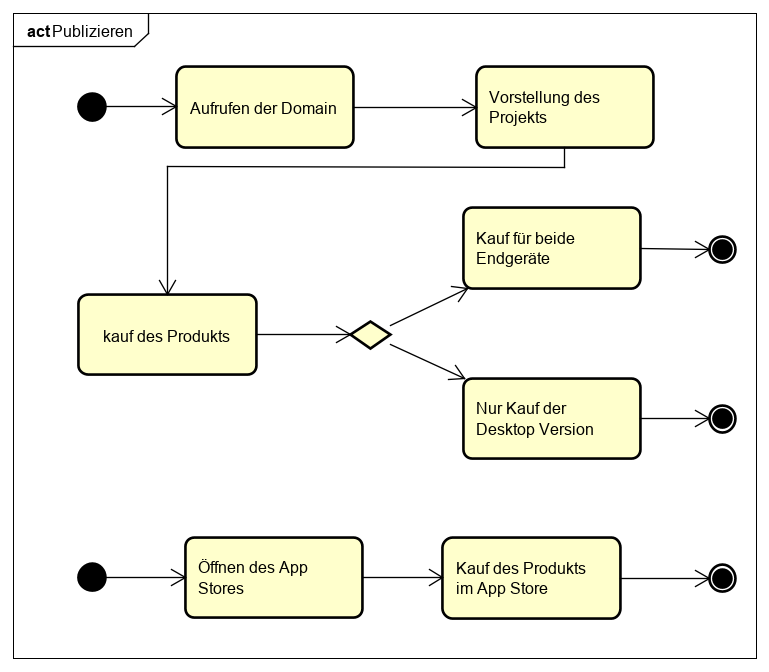
\includegraphics[width= 0.9\linewidth]{diagramms/activity/Publizieren.png}
	\caption{Aktivitätsdiagramm Publizierung}
\end{figure}
\newpage
\begin{indentE}\mbox{}
	\paragraph{/LF3110/ Website erstellen}\mbox{}\\
	Es wird eine Webseite erstellt, auf welche das Produkt vorgestellt wird. Außerdem soll diese dem Besucher das Projektteam und den Auftraggeber näher bringen, auf einer eigenen About-Seite. Diese Webseite wird dann auf einen Hosting-Provider hochgeladen, von wo sie mit einer Domain aufgerufen werden kann.
	\UseCase{
		{Publizierung}
		{/LF3110/ Website erstellen}
		{Publizierung}
		{Es wird eine Webseite erstellt, auf welche das Produkt publiziert werden soll. Diese soll außerdem auf das Projektteam aufmerksam machen und über das Internet mit einer Domain erreichbar sein.}
		{Das Produkt soll auf einer Webseite publiziert werden, und den potenziellen Kunden das Projektteam näher gebracht werden.}
		{Das Produkt ist im Internet auffindbar}
		{Benutzer, Projektteam (Auftraggeber + Auftragnehmer)}
		{Produktinformationen, Projektteam}
		{Das Produkt kann nicht über eine Webseite aufgefunden werden.}
		{Das Produkt ist über ein Webseite auffindbar}
		{hoch}
		{gering}
		{Must Have}
	}
	\paragraph{/LF3120/ Produkt auf Webseite veröffentlichen}\mbox{}\\
	Das Produkt muss auf ihrer eigenen Webseite /LF2060/ publiziert werden. Diese besitzt eine eigne Seite für den Download der Software. Dort kann man die App und Desktop Version für 5€ kaufen und die Desktop Version einzeln für 3€.
	\UseCase{
		{Publizierung}
		{LF3120/ Produkt auf Webseite veröffentlichen}
		{Publizierung}
		{Das Produkt soll von der Webseite gedownloadet werden können. Dabei soll die App und Desktop Version für 5 € gemeinsame und die Desktop Version einzeln für 3€ angeboten werden.}
		{Das Produkt muss für den potenziellen Kunden erwerbbar sein}
		{Das Produkt kann auf der Webseite automatisiert verkauft werden}
		{potenzieller Kunde}
		{Zahlungsinformationen, Produkt (als Download)}
		{Das Produkt ist für den potenziellen Kunden nicht erwerbbar}
		{Das Produkt kann auf der Webseite verwirtschaftet werden}
		{hoch}
		{mittel}
		{Must Have}
	}
	\paragraph{/LF3210/ Produkt auf Play Store veröffentlichen}\mbox{}\\
	Die Android App soll auf dem Google Play Store hochgeladen werden und dort für eine Preis von 3€ verkauft werden. Dafür muss ein Google Developer Account erstellt werden, um diese hochzuladen.
	\UseCase{
		{Publizierung}
		{/LF3210/ Produkt auf Play Store veröffentlichen}
		{Publizierung}
		{Die App-Version wird auf dem Play Store veröffentlicht, wo sie für 3€ erwerbt werden kann.}
		{Es soll die potenzielle Kundschaft erhöht werden, indem ie App-Version auch auf dem Play-Store verfügbar ist.}
		{Es wird eine größter Kundschaft(Android) angesprochen}
		{potenzielle Kunden}
		{App-Version(als Download)}
		{Der Erwerb wird nicht auf dem Play Store angeboten.}
		{Der Erwerb ist über den Play Store möglich}
		{mittel}
		{gering}
		{Should Have}
	}
	\paragraph{/LF3220/ Produkt auf App Store veröffentlichen}\mbox{}\\
	Die iOS App kann auf dem Apple App Store hochgeladen werden und dort für 3€ verkauft werden.
	\UseCase{
		{Publizierung}
		{/LF3220/ Produkt auf App Store veröffentlichen}
		{Publizierung}
		{Die App-Version wird auf dem App Store veröffentlicht, wo sie für 3€ erwerbt werden kann.}
		{Es soll die potenzielle Kundschaft erhöht werden, indem ie App-Version auch auf dem App Store verfügbar ist.}
		{Es wird eine größter Kundschaft(iOS) angesprochen}
		{potenzielle Kunden}
		{App-Version(als Download)}
		{Der Erwerb wird nicht auf dem App Store angeboten.}
		{Der Erwerb ist über den App Store möglich}
		{mittel}
		{mittel}
		{Nice to Have}
	}
\end{indentE}